% !TeX program = lualatex

%% We need to use lualatex to make some features of tikz-feynman work properly 

% Copyright (c) 2024-2025 Simon Crase

% Permission is hereby granted, free of charge, to any person obtaining a copy
% of this software and associated documentation files (the "Software"), to deal
% in the Software without restriction, including without limitation the rights
% to use, copy, modify, merge, publish, distribute, sublicense, and/or sell
% copies of the Software, and to permit persons to whom the Software is
% furnished to do so, subject to the following conditions:

% The above copyright notice and this permission notice shall be included in all
% copies or substantial portions of the Software.

% THE SOFTWARE IS PROVIDED "AS IS", WITHOUT WARRANTY OF ANY KIND, EXPRESS OR
% IMPLIED, INCLUDING BUT NOT LIMITED TO THE WARRANTIES OF MERCHANTABILITY,
% FITNESS FOR A PARTICULAR PURPOSE AND NONINFRINGEMENT. IN NO EVENT SHALL THE
% AUTHORS OR COPYRIGHT HOLDERS BE LIABLE FOR ANY CLAIM, DAMAGES OR OTHER
% LIABILITY, WHETHER IN AN ACTION OF CONTRACT, TORT OR OTHERWISE, ARISING FROM,
% OUT OF OR IN CONNECTION WITH THE SOFTWARE OR THE USE OR OTHER DEALINGS IN THE
% SOFTWARE.

\documentclass[]{article}

\usepackage{caption}
\usepackage{subcaption}
\usepackage{graphicx}
\usepackage{float}
\usepackage{url}
\usepackage{amsmath}
\usepackage{amssymb}
\usepackage{amsthm}
\usepackage{tocloft}
\usepackage{cancel}
\usepackage{thmtools}
\usepackage{gensymb}
\usepackage{braket}
\usepackage{bm}
\usepackage[compat=1.0.0]{tikz-feynman}
\usepackage{tikz}
\usepackage{pgfplots}
\usepackage{mathtools}
\usepackage{color}
\usepackage{colortbl}
\usepackage[toc,nonumberlist]{glossaries}
\usepackage{glossaries-extra}

\newcommand\numberthis{\addtocounter{equation}{1}\tag{\theequation}}
\newcommand{\Lagr}{\mathscr{L}}
\newtheorem{thm}{Theorem}
\newtheorem{defn}[thm]{Definition}
\newtheorem{cor}[thm]{Corollary}
\newtheorem{lemma}[thm]{Lemma}
\graphicspath{{figs/}}
\widowpenalty10000
\clubpenalty10000
\setcounter{tocdepth}{2}
\tikzfeynmanset{compat=1.0.0}

%opening
\title{Theoretical Minimum\\Particle Physics 3\\Supersymmetry \& Grand Unification}
\author{Simon Crase (compiler)\\simon@greenweaves.nz}
\makeglossaries
\loadglsentries{glossary-entries}
\begin{document}

\maketitle

\begin{abstract}
	These are my notes for the \emph{New Revolutions in Particle Physics 3--Supersymmetry and Grand Unification} lectures from Leonard Susskind's \emph{Theoretical Minimum} series\cite{susskind2007theoretical}. 
	
	Disclaimer: I have created these notes as an aide-m\'emoire for my own use; if you find them useful, you are welcome, but I'd appreciate hearing from you. They are not intended 
	as a substitute for listening to the lectures. The intellectual property for all material derived from the lectures belongs, of course, to Professor Susskind; any mistakes, however, are my own.
	
\end{abstract}

\tableofcontents
\listoffigures
\listoftables
\listoftheorems

\section{Renormalization  and dimensional analysis}\label{sect:renormalization}

\subsection{Renormalization}

Most of the basic ideas of this quarter originated out of questions having to do with renormalization -- sometimes puzzles, sometimes useful observations about the renormalization of the standard model. I thought it would be a good idea to explain what renormalization is. It  is a combination of two things:
\begin{itemize}
	\item Learning how to eliminate out of the description of physics things arising from distances that are so small that they are irrelevant to the questions you are asking
	\item Learning how to think about how dimensional analysis tells you how to answer some of the difficult questions of quantum field theory field theory that have to do with distances much smaller than you might be interested in.
\end{itemize}

Examples of getting rid of things that are too small to be of interest.
\begin{itemize}
	\item Studying the nucleus as protons and neutrons instead of quarks. Use \gls{gls:QCD} to figure out properties of protons and neutrons and their forces. Nucleons move slowly, so we can ignore relativity. Nucleus can be described by the non-relativistic theory of neutrons and protons. All we need from quark theory is to find out what the properties of protons and neutrons are: masses, spins, and the forces between them.
	\item For atoms, you might not be particularly interested in what makes up the nucleus. You use nuclear physics to calculate the properties of nuclei--which nuclei exist, their masses, and charges. Now we can forget protons and neutrons, but we need electrons.
	\item Now move on to atoms and forget their contents.
\end{itemize}

At each stage we eliminated the things that are smaller than we are really interested. The result is a coarse-grained description that is less accurate but more useful for our purposes.

The same thing is true in field theory. Each possible wavelength represents a degree of freedom. In describing things at one length scale we don't want to deal with shorter scales. We find a way to sum up the shorter stuff and replace by effective new parameters. That is all that renormalization is (plus some dimensional analysis).

\subsubsection{Example: atoms and atomic forces--going from atoms to molecules.}

Or going from nuclei + electrons to atoms, and how you deal with atomic forces: where do atomic forces come from? This isn't usually thought of as renormalization, but it is renormalization. Getting rid of the very small degrees of freedom, and also the very fast degrees of freedom: small usually goes with fast. The smaller a system is, typically the faster its motion is. So we are getting rid of small things and fast things.

Consider two atoms, each including a cloud of electrons. We want to get rid of the cloud of electrons, and all that very complicated stuff. We'd like to replace Figure \ref{fig:3-2-atoms} with two simple atoms with forces between them. The advantage is that the electrons are very fast compared to the nuclei. Nuclei are very heavy, starting at 2000 times the mass of the electron, so we could almost think of atom as a bowling ball with little flies surrounding it.

\begin{figure}[H]
	\begin{center}
		\caption{Two atoms with clouds of electrons}\label{fig:3-2-atoms}
		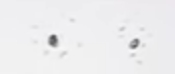
\includegraphics[width=0.5\textwidth]{3-2-atoms}
	\end{center}
\end{figure}

First approximation: the atoms are so heavy that they don't move at all. We want to calculate the effective potential between the two nuclei, in a way that gets rid of the electrons. Start by writing down Hamiltonian (ignore relativity, and some factors of $2\pi$).

\begin{align*}
	E=& \underbrace{\frac{P_1^2}{2M} + \frac{P_2^2}{2M} + \frac{e^2}{R_{12}}}_\text{protons} + \underbrace{\sum_i \frac{q_i^2}{2m} + \sum_{i,j}\frac{e^2}{r_{ij}}- \sum_i \frac{e^2}{R_{1i}} - \sum_i \frac{e^2}{R_{2i}}}_\text{things that involve electrons} \numberthis \label{eq:hamiltonian:H2}
\end{align*}

Intuitively there are two time scales here:
\begin{itemize}
	\item slow for nuclei, which are heavy;
	\item fast for electrons, which are a blur.
\end{itemize}

We'd like to get rid of the blur of electrons. This is easy to do \emph{in principle.} Take everything in the Hamiltonian that involves electrons; group them and think of them as the Hamiltonian for the electrons alone. Since the nuclei move slowly compared to electrons, treat them as fixed: to a first approximation nuclei are stationary.

To a first approximation fix the protons and treat the Hamiltonian as being for electrons in a fixed background from nuclei. We solve the Schr\"odinger equation for the lowest energy eigenvalue, $E_{electrons}(R_1,R_2)$. Then (\ref{eq:hamiltonian:H2}) becomes:


\begin{align*}
E=& \underbrace{\frac{P_1^2}{M} + \frac{P_2^2}{M} + \frac{e^2}{R_{12}}}_\text{protons} +\underbrace{ E_{electrons}(R_1,R_2)}_\text{Part of potential energy}\\
=& \frac{P_1^2}{M} + \frac{P_2^2}{M} + \frac{e^2}{R_{12}}+ E_{electrons}(R_1-R_2)
\end{align*}

We don't have to think about electrons again. All renormalization is based on this idea: getting rid of fast degrees of freedom, and replacing them with a renormalized Hamiltonian. 

What do we get rid of in Quantum Field Theory? Things associated with very small distances, or things associated with high frequencies, or very short wave lengths (high energies). But first let's take a break and work on dimensional analysis.

\subsection{Dimensional Analysis}

In physics we have three scales, distance, time, and mass, and we can get rid of two of them by setting:
\begin{align*}
	c=&1\\
	\hslash=& 1
\end{align*} 
but we still need one dimension, which we will take to be a length (we could have used a time, or a mass). With the above units we have: 

\begin{align*}
	[m] =& [E]	= [P]\\
	[l] =& [t]	= \frac{1}{[m]}
\end{align*}

\subsection{Vacuum energy renormalization}
\subsubsection{A typical quantum field theory}

Renormalizing a scalar field $\Phi$. It has a Lagrangian, from which we derive Feynman diagrams. Our Lagrangian is:

\begin{align*}
	\mathcal{L} =& (\partial_\mu \Phi)^2 - V(\Phi) \text{, which we use to determine the \emph{action}}\\
	S =& \int d^4 x \mathcal{L} \text{, which has the same units as $\hslash=1$}
\end{align*}

This means that $\mathcal{L}$ has dimensions $[l^{-4}]$

\begin{align*}
	[(\frac{\partial \Phi}{\partial x})^2]=l^{-4} \text{, whence}\\
	[\Phi] = l^{-1}
\end{align*}

\subsubsection{Feynman diagrams}

We imagine that the potential is something like:
\begin{align*}
	V(\Phi) =& \frac{m^2}{2} \Phi^2 + g \Phi^3 + \lambda \Phi^4 \numberthis \label{eq:potential}
\end{align*}
Since $[\Phi] = l^{-1}$ we can read off the dimensions of the coefficients:
\begin{itemize}
	\item $m$--mass;
	\item $g$--mass;
	\item $\lambda$--dimensionless. Dimensionless coupling constants are very important in renormalization theory.
\end{itemize}

Feynman diagrams are built out of two types of elements:
\begin{itemize}
	\item vertices, read off from V--(\ref{eq:potential})-- see Figure \ref{fig:3-1-feynman-vertices}
	\item propagators: represent motion from one point to another--Figure \ref{fig:3-1-feynman-propagator}.
\end{itemize}

\begin{figure}[H]
	\begin{center}
		\caption{Elements of a Feynman diagram}
		\begin{subfigure}[t]{0.45\textwidth}
			\caption{Feynman Vertices for (\ref{eq:potential}). Cross in left hand vertex indicates absorption/re-emission. A Feynman diagram has a value, which corresponds to the amplitude for a process to happen.}\label{fig:3-1-feynman-vertices}
			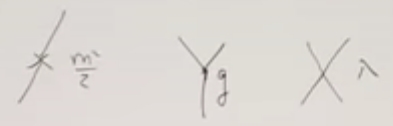
\includegraphics[width=\textwidth]{3-1-feynman-vertices}
		\end{subfigure}
		\begin{subfigure}[t]{0.45\textwidth}
			\caption{Propagator--amplitude that particle created at $x$ found at $y$. The line should not be read as a path along which particles moves, but rather as joining points where particle detected.}\label{fig:3-1-feynman-propagator}
			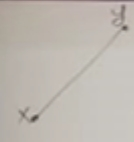
\includegraphics[width=\textwidth]{3-1-feynman-propagator}
		\end{subfigure}
	\end{center}
\end{figure}

\begin{itemize}
	\item We can represent the propagator is  $\braket{0|\bar{\Phi}(y)\Phi(x)|0}$: create at $x$, annihilate at $y$.
	\item Dimension of propagator is $[l^{-2}]$. If there is no mass, distance between $x$ and $y$ is the only length scale in the problem--$\frac{1}{\lVert x-y \Vert^2}$. 
	\item If $x$ and $y$ close, propagator blows up--this is the source of all divergences in \gls{gls:QFT}.
\end{itemize}

Everything else is just building up Feynman diagrams, calculating them, and interpreting them.

\subsubsection{Renormalization of Mass}

Let's start with renormalization, and how it works in this very simple context.
Let's start with renormalization of the mass. Notice that (\ref{eq:potential}) contains $m^2$ -- usually mass only appears as $\sqrt{m^2}$. This is connected with $E=\sqrt{p^2 + m^2}$. So what is renormalization of $m^2$? What does it mean, and how do we do it? In Figure \ref{fig:3-1-feynman-vertices} we see that the interpretation of a mass term is just a basic simple Feynman diagram, a vertex in the diagram where a particles is absorbed at a point and emitted from the same point. Does it have to be exactly the same point? If we have a microscope, an accelerator, which can resolve down to $10^{-17}m$, say, we aren't really interested in things that happen on smaller scales; so if we can find a process in nature that would mimic that vertex,  even if blurred, any process that absorbs and re-emits at a nearby point would be counted as part of mass term in an effective description in which we don't look too closely.

Are there any Feynman diagrams that we can build that will mimic a particle going in and a particle going out? We will build it out of the $\Phi^4$ vertex in Figure \ref{fig:3-1-feynman-vertices}, the $\lambda$ vertex--see Figure \ref{fig:3-1-feynman-mimic}.


\begin{figure}[H]
	\caption{Mimicking the Vertex}\label{fig:mimicking:vertex}
	\begin{subfigure}[t]{0.32\textwidth}
		\caption{Particle emitted and returns to same point: scale so small we don't notice. Particle isn't going anywhere!}\label{fig:3-1-feynman-mimic}
		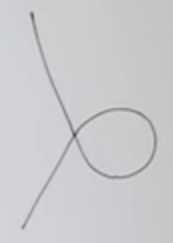
\includegraphics[width=\textwidth]{3-1-feynman-mimic}
	\end{subfigure}
	\begin{subfigure}[t]{0.32\textwidth}
		\caption{Amplitude following cut-off. We have reinstated $\lambda$ from $\Phi^4$ term.}\label{fig:3-1-cutoff}
		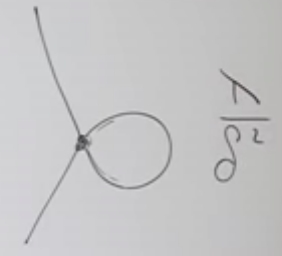
\includegraphics[width=\textwidth]{3-1-cutoff}
	\end{subfigure}
		\begin{subfigure}[t]{0.32\textwidth}
		\caption{Original mass term}\label{fig:3-1-original}
		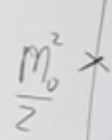
\includegraphics[width=\textwidth]{3-1-original}
	\end{subfigure}
\end{figure}

We saw in Figure \ref{fig:3-1-feynman-propagator} that the propagator has amplitude:
\begin{align*}
	\braket{0|\bar{\Phi}(y)\Phi(x)|0}=&\frac{1}{|x-y|^2}\text{, which blows up to $infty$}
\end{align*}

Let us introduce a cut-off, saying that we are not interested in scales smaller than $\delta$; we smear the point over $\delta$--Figure \ref{fig:3-1-cutoff}. What is the amplitude in this approximation for a particle to come in, be absorbed, and re-emitted? There are two ways to make this happen. Figure \ref{fig:3-1-original} shows the original mass term. If we include Figure \ref{fig:3-1-cutoff} we see that the effect of ignoring terms smaller than $\delta$ is to increase the effective mass: the amplitude becomes $\frac{m_0^2}{2}+\frac{1}{\delta^2}$.  \emph{This is what we'd see in the laboratory if our resolution isn't high enough to resolve lengths less than $\delta$.}  

But we haven't finished. We haven't evaluated every possible Feynman diagram that can go into this. Let's do another Feynman diagram for the same thing. Figure \ref{fig:particles3-another-Feynman} depicts a particles going in and out, and something happening in the centre. What if the centre has size $\approxeq \Delta$? Can we integrate it out?

\begin{figure}[H]
	\begin{center}
		\caption{More diagrams from Figure \ref{fig:mimicking:vertex}}
		\begin{subfigure}[t]{0.45\textwidth}
			\caption{Another Diagram. Particle is absorbed where the heavy dot is. We need to integrate over all the places where it could be re-emitted. This derives from the third part of Figure \ref{fig:3-1-feynman-vertices}--4 things coming together at a vertex.}\label{fig:particles3-another-Feynman}
			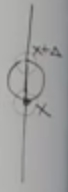
\includegraphics{particles3-another-Feynman}
		\end{subfigure}
		\begin{subfigure}[t]{0.45\textwidth}
			\caption{Diagram giving $\lambda^4$}\label{fig:particles3-yet-another-Feynman}
			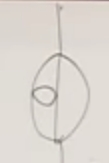
\includegraphics{particles3-yet-another-Feynman}
		\end{subfigure}
	\end{center}
\end{figure}

Coefficient is of order $\lambda^2$, so it is a second order Feynman diagram. It also has three propagators, each with coefficient $\frac{1}{\Delta^2}$, so $\frac{1}{\Delta^6}$. We need to integrate over all $\delta s$ 

\begin{align*}
	\lambda^2 \int_{\delta}^\infty \frac{1}{\Delta^6} d^4 \Delta \propto& \frac{\lambda^2}{\delta^2} \text{, by dimensional analysis.}
\end{align*}

There are many other Feynman diagrams, which will also contribute higher powers of $\lambda$. There is an infinite series of terms of order $\frac{1}{\Delta^2}$, with higher powers of $\lambda$. There are other terms that we haven't used, from $\Phi^3$.

Consider:
\begin{align*}
	\int_{\delta}^{\infty} \frac{d \delta}{\delta} =& - \log(\delta)
\end{align*}
Dimensional analysis would suggest this is dimensionless, but we have to be careful as it is a divergent integral. In dimensional analysis, an integral with  the same number of powers of $\delta$ in the numerator and denominator is always a logarithm. Since log is always $\log\frac{...}{scale}$ we treat as dimensionless.

Consider Figure \ref{fig:particles3-1-two-cubic-vertices}. There are two propagators, giving $\frac{1}{\Delta^4}$.
\begin{figure}[H]
	\begin{center}
		\caption{Two cubic vertices, with 3 particles at each vertex.}\label{fig:particles3-1-two-cubic-vertices}
		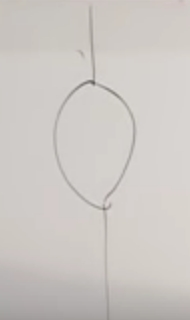
\includegraphics{particles3-1-two-cubic-vertices}
	\end{center}
\end{figure}

We have (keeping lower point fixed):
\begin{align*}
	\int_{\delta}^{\infty} \frac{g^2}{\Delta^4} d^4 \Delta =& g^2 \log(\delta)
\end{align*}

When $\delta$ is small, $\frac{1}{\delta^n}$ dominates $\log(\delta)$.

Note that $[g^2] = [m^2]$.

That is the idea of mass renormalization.

\subsubsection{Renormalization of $\lambda$}\label{sect:renormalization:lambda}

It's not just mass that gets renormalized: every term in the Lagrangian can get renormalized.

From an operational point of view, $\lambda \Phi^4$ is nothing but two particles being absorbed and re-emitted--Figure \ref{fig:lambda:phi:4}. If everything happens on a scale that is too small to see, we lump it in to $\lambda \Phi^4$. Now Figure \ref{fig:lambda:phi:4x} will also contribute a renormalzation to $\lambda \Phi^4$.

\begin{figure}[H]
	\begin{center}
		\caption{Renormalization of $\lambda \Phi^4$}
		\begin{subfigure}[t]{0.45\textwidth}
			\caption{Feynman Diagram for $\lambda \Phi^4$}\label{fig:lambda:phi:4}
			\feynmandiagram[horizontal=i1 to f1]{
				i1--[fermion]a--i2,
				f1--[fermion]a--f2
			};
		\end{subfigure}
		\begin{subfigure}[t]{0.45\textwidth}
			\begin{center}
				\caption{This will also contribute a renormalization to $\lambda \Phi^4$}\label{fig:lambda:phi:4x}
				\feynmandiagram[horizontal=i1 to i2]{
					a--[quarter right]b
					--[quarter right]c
					--[quarter right]d
					--[quarter right]a,
					i1--[fermion]a,
					i2--[fermion]a,
					c--[fermion]o1,
					c--[fermion]o2
				};
			\end{center}
		\end{subfigure}
	\end{center}
\end{figure}

Each one of these terms can be renormalized. The effect of very small scale physics, when you sum it up and take it into account the way we did with the electron, we find some description that doesn't involve these microscopic degrees of freedom. \emph{The parameters of the theory that you measure are not the same as the ones you input to the theory!}

\subsubsection{Renormalization of the mass of a Fermion}


You might expect the theory to work the same for Fermions, but it doesn't. Fermions are better behaved than Bosons, which are badly behaved in the following sense. Imagine that the cutoff distance is very, very small, e.g. the Planck scale. The $\delta \approx l_p = \sqrt{\frac{\hslash G}{\c{^3}}}$--20 order of magnitude smaller than a proton, 16 orders of magnitude smaller than the resolution of our best accelerators! If we are working on the Higgs Boson, we'd need the expressions in (\ref{eq:sum:lambdas}) to cancel to 34 digits, leaving the answer in the 35th. This is known as the "fine-tuning problem of the Higgs Boson".
\begin{align*}
	\frac{m_0^2}{2} + \frac{\lambda}{\delta^2} +  + \frac{\lambda^2}{\delta^2}  + \frac{\lambda^3}{\delta^2} =& \frac{m^2}{2}\numberthis\label{eq:sum:lambdas}
\end{align*}

Let's recall what we know about the mass term of the Higgs Boson. The Higgs field has a potential that looks like Figure \ref{fig:higgs-potential}. Near the origin it looks like $\Phi^2$, but with a negative coefficient ($m_0^2$ can be negative!). We assume that $\lambda<1$, as otherwise sequence of power would be intractable. Assume $\lambda$ is modestly small, but not humungously so. Experimentally we know it's about $1\%$.

\begin{figure}[H]
	\caption[Higgs potential]{Higgs potential after \cite{susskind2010standard}: Near the origin it looks like $\Phi^2$, but with a negative coefficient }\label{fig:higgs-potential}
	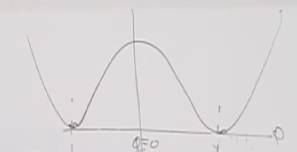
\includegraphics{higgs-potential}
\end{figure}

\begin{align*}
	V(\Phi) =& - \frac{\mu^2}{2} \Phi^2 + \lambda \Phi^4\\
	\Phi_{min}^2 =& f^2 = \frac{\mu_2}{\lambda} \numberthis \label{eg:higgs:minimum}
\end{align*}

Now experimentally we know that $f\approxeq200GeV$, and $\lambda$ is of order 1, so $\mu^2$ is of order 200GeV, yet it is computed by (\ref{eq:sum:lambdas}), every term being 38 orders of magnitude bigger! This is known as the "fine-tuning problem", or the "gauge hierarchy problem", or the "hierarchy problem", the hierarchy being the hierarchy of mass scales from Planck scale to the scale of ordinary particle physics. There are many finely tuned pieces, which have to add up to something small. We know that this is ridiculous: what do we do about that.

There is no such problem with other particles in the Standard Model. Why doesn't the electron have the same kind of problem? Let's talk about Fermions.

The mass term of a Fermion involves the mass, not the mass squared. The Lagrangian contains a term $m \bar{\Psi} \Psi$. Figure \ref{fig:Fermion:feynman} shows the Feynman diagram. What kind of thing could renormalize electron?

\begin{figure}[H]
	\begin{center}
		\caption{Feynman diagram for $m \bar{\Psi} \Psi$}
		\begin{subfigure}[t]{0.3\textwidth}
			\caption{$m \bar{\Psi} \Psi$ flips helicity}\label{fig:Fermion:feynman}
			\feynmandiagram[vertical=b to a]{
				a--[fermion,edge label=L]b
				--[fermion,edge label=R]c
			};
		\end{subfigure}
		\begin{subfigure}[t]{0.3\textwidth}
				\caption{Emit scalar boson}\label{fig:emit:scalar}
				\feynmandiagram[vertical=b to a]{
					a--[fermion,edge label=L]b
					--[fermion,edge label=R]c,
					b--[scalar]d
				};
		\end{subfigure}
		\begin{subfigure}[t]{0.3\textwidth}
			\caption{Emit gauge boson}\label{fig:emit:gauge}
			\feynmandiagram[vertical=b to a]{
				a--[fermion,edge label=L]b
				--[fermion,edge label=L]c,
				b--[photon]d
			};
		\end{subfigure}
	\end{center}
\end{figure}

We recall that $m \bar{\Psi} \Psi$ always absorbs a left handed particle and emits right handed, or vice versa[find reference to this in earlier lecture]--it flips helicity. What sort of thing could renormalize the electron? We could emit a boson, Figures \ref{fig:emit:scalar} and \ref{fig:emit:gauge}. In QED the only thing that can happen is to emit a photon, Figure \ref{fig:emit:gauge}. What happens to the handedness of the electron when it emits a gauge boson? The answer is nothing: the handedness doesn't change: The emission of a gauge boson doesn't flip helicity--Figures \ref{fig:emit:gauge:no:flip}.
[Work this out from Lagrangian]
\begin{figure}[H]
	\begin{center}
		\caption{Emission of a gauge boson doesn't flip helicity}\label{fig:emit:gauge:no:flip}
		\begin{subfigure}[t]{0.3\textwidth}
			\caption{Emit gauge boson}\label{fig:emit:gauge:LL}
			\feynmandiagram[vertical=b to a]{
				a--[fermion,edge label=L]b
				--[fermion,edge label=L]c,
				b--[photon]d
			};
		\end{subfigure}
		\begin{subfigure}[t]{0.3\textwidth}
			\caption{Emit gauge boson}\label{fig:emit:gauge:RR}
			\feynmandiagram[vertical=b to a]{
				a--[fermion,edge label=R]b
				--[fermion,edge label=R]c,
				b--[photon]d
			};
		\end{subfigure}
	\end{center}
\end{figure}

What about a scalar boson? It turns out they do flip--Figure \ref{fig:emit:scalar:flip}.
\begin{figure}[H]
	\begin{center}
		\caption{Emission of a scalar boson does flip helicity}\label{fig:emit:scalar:flip}
		\begin{subfigure}[t]{0.3\textwidth}
			\caption{Emit gauge boson}
			\feynmandiagram[vertical=b to a]{
				a--[fermion,edge label=L]b
				--[fermion,edge label=R]c,
				b--[scalar]d
			};
		\end{subfigure}
		\begin{subfigure}[t]{0.3\textwidth}
			\caption{Emit gauge boson}
			\feynmandiagram[vertical=b to a]{
				a--[fermion,edge label=R]b
				--[fermion,edge label=L]c,
				b--[scalar]d
			};
		\end{subfigure}
	\end{center}
\end{figure}

We'll look at processes that can renormalize the mass of an electron. Suppose that electron starts with no mass. In the Boson case, if particle starts with no mass it gets humongous contribution from the $\lambda s$ and $\delta s$ in (\ref{eq:sum:lambdas}). So renormalized mass is independent of original. Now let's take the electron. It could emit and absorb a photon--Figure \ref{fig:emit:absorb:photon}. Now, by definition, a mass term is recognized as an amplitude to change from L to R or vice versa--an oscillation. Can this happen, as in Figure \ref{fig:can:this:happen}? Photons can't do this. The conslusion is that in QED, or any theory with gauge bosons only, electrons get no mass renormalization at all, so the correction to a massless electron would be zero. In pure QED (not the Standard Model) a massless electron is a consistent thing. What about scalar bosons? Figure \ref{fig:higgs:doesnt:help} shows why they don't help. No matter how complex the Feynman diagram, it is always going to involve an even number of vertices.

\begin{figure}[H]
		\caption{Electron emits and absorbs boson}\label{fig:emit:absorb:photon}
		\begin{subfigure}[t]{0.3\textwidth}
			\caption{Emit gauge boson}
			\feynmandiagram[vertical=b to a]{
				a--[fermion]b
				--[fermion]c
				--[fermion]d,
				b--[photon,half left,looseness=1.5]c
			};
		\end{subfigure}
		\begin{subfigure}[t]{0.3\textwidth}
			\caption{Can this happen? Is there any way to go from L to R?}\label{fig:can:this:happen}
			\feynmandiagram[vertical=b to a]{
				a--[fermion,edge label=L]b
				--[fermion]c
				--[fermion,edge label=R]d,
				b--[photon,half left,looseness=1.5]c
			};
		\end{subfigure}
		\begin{subfigure}[t]{0.3\textwidth}
			\caption{Scalar bosons don't help, as the helicity gets flipped twice}\label{fig:higgs:doesnt:help}
			\feynmandiagram[vertical=b to a]{
				a--[fermion,edge label=L]b
				--[fermion,edge label=R]c
				--[fermion,edge label=L]d,
				b--[scalar,half left,looseness=1.5]c
			};
		\end{subfigure}
	\end{figure}

Can you ever get a shift in the mass of an electron in QED? Yes--if you \emph{start} with a mass. Figure \ref{fig:renormalization:massive:electron} shows a mass insertion which takes electron from $L$ to $R$. 
 
\begin{figure}[H]
	\caption{Mass Renormalization of massive electron via $ \bar{\Psi} \Psi$}\label{fig:renormalization:massive:electron}
	\feynmandiagram[vertical=e to a]{
		a--[fermion,edge label=L]b
		 --[fermion,edge label=L]c[particle=\( \bar{\Psi} \Psi  \)]
		 --[fermion,edge label=R]d
		 --[fermion,edge label=R]e,
		 b--[photon,half left,looseness=3.0]d
	};
\end{figure}

The value of this Feynman diagram contains three terms:
\begin{itemize}
	\item the electric charge twice;
	\item the original starting mass;
	\item more complicated terms from additional photons.
\end{itemize}

\begin{align*}
	m =& m_0 + m_0 e^2 + m_0 e^4 +...
\end{align*}

So if the starting mass is small it will remain small. For reasons we don't understand the mass is small, and the corrections are even smaller. We don't have a fine-tuning problem. Fermions are better behaved than scalar particles.

What about gauge bosons? They have the same property: if they start massless they remain massless to all orders. There is therefore only one fine-tuning problem, the fine-tuning problem of the Higgs Boson. Get that one right and all the others are alright, as their masses arise from shifting of the Higgs field. If $f$ is controlled (\ref{eg:higgs:minimum}), then all other masses are controlled. The only really crazy fine-tuning in the Standard Model is  $f$, which has to be 38 order of magnitude smaller than we'd expect from (\ref{eq:sum:lambdas}). This is the great puzzle that super-symmetry and other theories are intended to address. Roughly speaking we ask whether there is any theory where the Higgs mass isn't driven to enormous values by renormalization.

\subsubsection{Renormalization of vacuum energy}\label{sect:vacuum:energy:renormalization}
There is one other extreme fine-tuning problem, but it only comes in to play when we start thinking about gravity. It is the problem of renormalization of vacuum energy.

For most physics the vacuum energy isn't a problem, as it is an additive constant: normally when we add a particles we care only that it adds the right energy. Energy differences are all that is important. Don't think of the energy of an electron, think of the energy we have to add to the vacuum. Who cares if we add a large amount of energy to the vacuum, as long as everything is shifted with it? 

Vacuum is renormalized by diagrams that have no inputs and no outputs. Figure \ref{fig:particles3-1-5-4-theory} shows a such a diagram from the 5-4 theory
\begin{figure}[H]
	\begin{center}
		\caption{5-4 theory: value $\lambda \frac{1}{\delta^2} \frac{1}{\delta^2}= \frac{\lambda}{\delta^4}$}\label{fig:particles3-1-5-4-theory}
		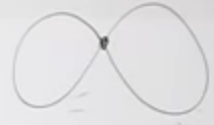
\includegraphics{particles3-1-5-4-theory}
	\end{center}
\end{figure}

There are more complicated diagrams. Vacuum energy gets renormalized, so if you want it to be zero you'd better fine-tune it to high precision. Who cares? We don't care \emph{until gravity becomes important}. The standard theory for gravity says that energy gravitates: this is connected to Dark Energy and the Cosmological constant; vacuum energy has to be fine-tuned to extremely high precision (123 decimal places).

The two fine-tuning problems are the biggest puzzles in particle physics at the present time. Maybe it will turn out that they are a misstatement of the problem, but it has been a long time and nobody knows what the solution is.
 
Supersymmetry is a potential problem to the fine tuning of the Higgs field, but it is not a potential solution to the fine-tuning of the cosmological constant.

If you believe \gls{gls:QFT} down to scales that are many times smaller than the weak interaction scale, but only is we can solve renormalization problems at smaller scales. This section deals with a lower bound the the problems. They could be bigger.

In order to cancel terms in (\ref{eq:sum:lambdas}), terms need to be very closely balanced. matching them is what Supersymmetry does. The simplest possible Feynman diagrams for Fermions have negative energy, the simplest for Bosons have positive. In principle if they had exactly the same mass they could cancel each other in the vacuum energy
	
\section{Fermions and bosons}

\subsection{Difference between Fermions and bosons}

Supersymmetry has to do with Fermions and Bosons, and their symmetries. We will talk again about Fermions and Bosons; I want to tell you some odd and peculiar facts about Fermions, but, before that, we'll look at rotations in space.

Normally we are told that a rotation of $2\pi$ is equivalent to no rotation at all, but it is not true.

\begin{thm}[Rotation by $4\pi$ is equivalent to no rotation at all]
	Take a box, put a basketball in, and connect it to the walls with flexible but unbreakable strings. A rotation by $2\pi$ tangles the strings; a rotation by $4\pi$ is equivalent to no rotation.
\end{thm}

Imagine that we have a particle, a Fermion or a Boson. We are interested in the spin of the particle only, and the spin is described by a quantum state $\bra{s}$. What happens to the state when you rotate the particle by $2\pi$?

How would you rotate an electron by $2\pi$?

\begin{itemize}
	\item apply strong magnetic field and rotate magnetic field around, or;
	\item use field to precess particle.
\end{itemize}

What happens to the state when you rotate the particle by $2\pi$? Normally we'd expect it to come back to itself, but we know that $2\pi$ is not the identity. Perhaps it multiplies by a number, $\bra{s} \rightarrow \xi \bra{s}$. If we multiply by a phase, $\xi$, we won't be able to detect it. Multiplication by $4\pi$ squares phase, since it does nothing, so $\xi^2=1$, or $\xi=\pm1$.

\begin{align*}
	\ket{s} \rightarrow& +\ket{s} \text{, or}\\
	\ket{s} \rightarrow& -\ket{s}
\end{align*}

Can we detect this experimentally? It was long thought that we could not. If we take a family of electrons, all prepared identically, stick half into a magnetic field and rotate $2\pi$, we can't tell the two lots apart.

We can, however, do a 2 slit experiment\cite{aharonov1967observability}--Figure \ref{fig:particles3-2-2slit}.

\begin{figure}[H]
	\caption{A 2 slit experiment to detect rotation by $2\pi$. We feed the electrons through one by one, without looking to see which slit they go through, and we place a magnetic field behind each slit.}
	\begin{subfigure}[t]{\textwidth}
		\begin{center}
			\caption{There is a magnetic field behind each slit, which traps electron temporarily. While an electron is trapped we rotate one field or the other, so wave function may be multiplied by $-1$ which shifts the interference pattern by half a wavelength. If you rotate the whole setup, then you detect nothing. Also, if you rotate one beam by $4\pi$ you detect nothing.}\label{fig:particles3-2-2slit}
			\begin{tikzpicture}
				\draw (0,-3) -- (0,-1.1);
				\draw (0,-1.0) -- (0,-0.1);
				\draw (0,0) -- (0,2);
				\draw (3,-2)--(3,2);
				\draw[decorate,decoration={snake,amplitude=.8mm,segment length=2mm,post length=0mm}] (3,-1.1) -- (3,-0.1);
				\draw[dashed](-2,-0.05) -- (0,-0.05);
				\draw[dashed](-2,-1.05) -- (0,-1.05);
				\draw[dashed](0.5,-0.05) -- (3,-0.2);
				\draw[dashed](0.5,-1.05) -- (3,-0.2);
				\draw (0.5,-0.05) circle [radius=0.2] node {B};
				\draw (0.5,-1.05) circle [radius=0.2] node {B};
			\end{tikzpicture}
		\end{center}
	\end{subfigure}
	\hfill
	\begin{subfigure}[t]{0.45\textwidth}
		\begin{center}
			\caption{We create a superposition of two states, electron going through slit 1 or slit 2. In either case electron is in one box or the other.}\label{fig:particles3-2-2slit-wave-function-2-2slit}
				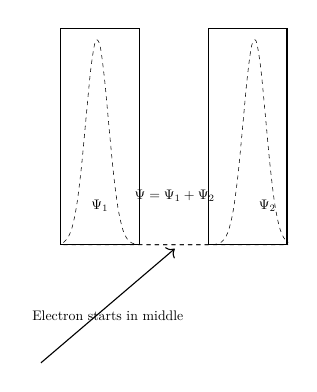
\begin{tikzpicture}[scale=0.5, transform shape]
				\newcommand\gauss[2]{1/(#2*sqrt(2*pi))*exp(-((x-#1)^2)/(2*#2^2))} 
				\begin{axis}[every axis plot post/.append style={
						mark=none,domain=-10:10,samples=50,smooth},
					clip=false,
					axis y line=none,
					axis x line=none,
					ymin=0,
					xtick=\empty,
					]
					\addplot [dashed,draw=black] {\gauss{-7}{1}};
					\addplot [dashed,draw=black] {\gauss{7}{1}};
				\end{axis}
				\draw (1.5,1) node {$\Psi_1$};
				\draw [draw=black] (0.5,0) rectangle (2.5,5.5);
				\draw (5.75,1) node {$\Psi_2$};
				\draw [draw=black] (4.25,0) rectangle (6.25,5.5);
				\draw [->] (0,-3)--(3.4,-0.1) node[midway,below] {Electron starts in middle};
				\draw (3.4,1.25) node {$\Psi=\Psi_1+\Psi_2$};
			\end{tikzpicture}
		\end{center}
	\end{subfigure}
		\hfill
	\begin{subfigure}[t]{0.45\textwidth}
		\begin{center}
			\caption{Now we rotate 2nd box by $2\pi$. The wave function for an electron changes sign, but this has no physical consequence on it own. For the superposition, if we rotate one electron wave function, we can never find the electron at the centre, as $\psi_1$ and $\psi_2$ will interfere. This is true for Fermions, with an odd wave function, but not for Bosons.}
			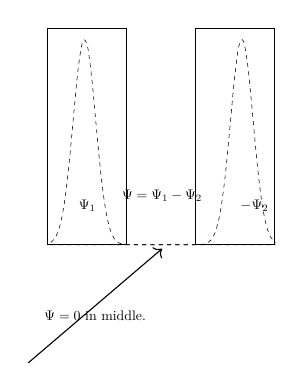
\begin{tikzpicture}[scale=0.5, transform shape]
				\newcommand\gauss[2]{1/(#2*sqrt(2*pi))*exp(-((x-#1)^2)/(2*#2^2))} 
				\begin{axis}[every axis plot post/.append style={
						mark=none,domain=-10:10,samples=50,smooth},
					clip=false,
					axis y line=none,
					axis x line=none,
					ymin=0,
					xtick=\empty,
					]
					\addplot [dashed,draw=black] {\gauss{-7}{1}};
					\addplot [dashed,draw=black] {\gauss{7}{1}};
				\end{axis}
				\draw (1.5,1) node {$\Psi_1$};
				\draw [draw=black] (0.5,0) rectangle (2.5,5.5);
				\draw (5.75,1) node {$-\Psi_2$};
				\draw [draw=black] (4.25,0) rectangle (6.25,5.5);
				\draw [->] (0,-3)--(3.4,-0.1) node[midway,below] {$\Psi=0$ in middle.};
				\draw (3.4,1.25) node {$\Psi=\Psi_1-\Psi_2$};
			\end{tikzpicture}
		\end{center}
	\end{subfigure}
\end{figure}

The experiment has been performed for Fermions (which get the minus sign), and Bosons (which don't). The result is also deeply embedded in the theory.

You cannot interfere an up spin with a down spin: you can only interfere things that are otherwise the same.

\subsection{Feynman Diagrams}

We'll be dealing with diagrams that are very simple. They are just Feynman diagrams in the vacuum, empty space, and they consist of nothing more complicated than a single closed loop. It could be an electron, Figure \ref{fig:particles3-2-loops}, or a photon, Figure \ref{fig:particles3-2-loops-boson}. This diagram controls, among other things, the amplitude that you start with nothing and get nothing. It is part of the vacuum structure. The diagram has a  value, which is a contribution to the vacuum energy. Just as Figure \ref{fig:particles3-2-loops-p} contributes to the energy of the particle, Figure \ref{fig:particles3-2-loops} and \ref{fig:particles3-2-loops-boson} contributes to the energy of the vacuum. Does it shift it up or down? We are going to find out that the answer is different for Fermions and Bosons.


\begin{figure}[H]
	\caption{A few Feynman diagrams}
	\begin{subfigure}[t]{0.3\textwidth}
		\caption{Fermion Closed Loop}\label{fig:particles3-2-loops}
		\feynmandiagram{
			b-- [fermion,half left]
			c-- [fermion,half left] b
		};
	\end{subfigure}
	\hfill
	\begin{subfigure}[t]{0.3\textwidth}
		\caption{Boson Closed Loop}\label{fig:particles3-2-loops-boson}
		\feynmandiagram{
			b-- [photon,half left]
			c-- [photon,half left] b
		};
	\end{subfigure}
	\hfill
	\begin{subfigure}[t]{0.3\textwidth}
		\caption{Loop which contributes to the energy of the particle}\label{fig:particles3-2-loops-p}
		\feynmandiagram[vertical=e4 to e1]{
			e1[particle=$e^-$]--[fermion]e2--[fermion]e3		--[fermion]e4[particle=$e^-$],
			e2--[photon,looseness=3.0,half left]e3
	};
	\end{subfigure}
\end{figure}



\begin{thm}[Contribution of loops to vacuum energy]\label{thm:contribution:loops}
	
	\begin{enumerate}
		\item The contribution to the vacuum energy of a loop of Bosons is positive;
		\item The contribution to the vacuum energy of a loop of Fermions is negative.
	\end{enumerate}
\end{thm}

\begin{proof}
	You can think of a loop as the production and annihilation of a particle-antiparticle pair, or as a single particle looping in space-time. The sign of a particle in a loop can be either positive or negative. What about two loops--Figures \ref{fig:two:loops:fermion} and \ref{fig:two:loops:boson}? This is the product of two separate loops. \begin{itemize}
		\item So if there is a plus sign for one loop, there will be a plus sign for the product.
		\item iI there is a minus sign for one loop, there will still be a plus sign for the product.
	\end{itemize} So there will  be a plus sign for the product either way.
	
	\begin{figure}[H]
		\caption{Two loops: each is a product of two separate loops.}\label{fig:two:loops}
		\begin{subfigure}[t]{0.45\textwidth}
			\begin{center}
				\caption{Two Fermion loops}\label{fig:two:loops:fermion}
				\feynmandiagram[scale=0.9, transform shape]{
					b-- [fermion,half left]
					c-- [fermion,half left] b
				};
				\feynmandiagram[scale=0.9, transform shape]{
					b-- [fermion,half left]
					c-- [fermion,half left] b
				};
			\end{center}
		\end{subfigure}
		\hfill
		\begin{subfigure}[t]{0.45\textwidth}
			\begin{center}
				\caption{Two Boson loops}\label{fig:two:loops:boson}
				\feynmandiagram[scale=0.9, transform shape]{
					b-- [boson,half left]
					c-- [boson,half left] b
				};
				\feynmandiagram[scale=0.9, transform shape]{
					b-- [boson,half left]
					c-- [boson,half left] b
				};
			\end{center}
		\end{subfigure}

	\end{figure}
	
	Let's assume our particles are Fermions: we will break the loop and look in the middle at t=0--Figure \ref{fig:two:loops:split}. 
		
	\begin{figure}[H]
		\caption{Breaking a Fermion loop and looking in the middle at t=0.}
		\begin{subfigure}[t]{0.45\textwidth}
			\caption{Two Fermion loops, split at t=0}\label{fig:two:loops:split}
				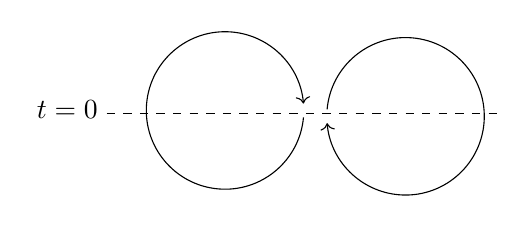
\begin{tikzpicture}
				\draw[->] (0.5,0) arc [radius=1, start angle=355, end angle= 5];
				\draw[->] (0.8,0.1) arc [radius=1, start angle=535, end angle= 185]; 
				\draw[dashed] (-2,0.05)--(3,0.05);
				\draw (-2.5,0.1)  node {$t=0$};
			\end{tikzpicture}	
		\end{subfigure}
		\hfill
		\begin{subfigure}[t]{0.45\textwidth}
			\caption{One Fermion loop, built by interchanging particles }\label{fig:two:loops:interchange}
			\begin{equation*}t=0
				\feynmandiagram[inline=(c.base),vertical=in1 to out1,scale=0.9, transform shape]{
					in1-- [fermion]c--[fermion]out1,
					in2-- [fermion]c--[fermion]out2,
					out1--[half left]in1,
					out2--[half right]in2,
				};
			\end{equation*}		
		\end{subfigure}
	\end{figure}

	\begin{itemize}
		\item What happens for amplitude of a system if we exchange two Bosons? We get a plus sign. 
		\item What happens for amplitude of a system if we exchange two Fermions? We get a minus sign. 
	\end{itemize}
	Now interchange particles, as in Figure \ref{fig:two:loops:interchange}.
	\begin{itemize}
		\item If we are dealing with Fermions we get a minus sign when we interchange the particles. We have gone from two loops (positive) to one loop, negative. A single loop for Fermions necessarily has a minus sign associated with it.
		\item If we are dealing with Bosons we get a plus sign. We have gone from two loops (positive) to one loop, also positive.
	\end{itemize} 
\end{proof}

The consequences are profound:
\begin{itemize}
	\item the contribution to the vacuum of a Boson loop is positive;
	\item the contribution to the vacuum of a Fermion loop is negative.
\end{itemize}
We have this strange puzzle about the vacuum energy, which was introduced in Section \ref{sect:vacuum:energy:renormalization}; it is extremely small, and we call it Dark Energy. The naive calculation in quantum field theory would give an answer 123 orders of magnitude larger. It is interesting that the answer can be positive or negative: it depends on all sorts of things, such as mass and charge. We can at least get positive and negative signs. The fact that they cancel to 123 order of magnitude is bizarre, butat least we have the possibility cancelling contributions. All things being equal, a boson and a fermion will give exactly the same contribution to the vacuum energy, except one with a plus sign and one with a minus sign.

That doesn't explain why the vacuum energy is zero, it may create a thought in your head: perhaps there is a lot of cancellation. To get an exact cancellation, we'd need for every boson with the same mass and same properties in every other respect, then we could conceive that the particles would cancel out the vacuum energy. That is one of the things that a supersymmetric theory can do: they can cancel out the contributions for the vaccum energy.

We know that there isn't an exact Boson for each Fermion and vice versa. For example, the electron: there isn't a Boson equivalent to the electron: if there were, the partners could be produced--Figure \ref{fig:partners}-- with exactly the same probability as an electron-positron pair--Figure \ref{fig:re:emit}. We know this isn't the case: Nature does not have a Boson$\leftrightarrow$Fermion symmetry. We know this because it doesn't happen in the laboratory; there is no Boson--Fermion reflection.  

\begin{figure}[H]
	\begin{center}
		\caption{Why there isn't a Boson equivalent to the electron}
		\begin{subfigure}{0.45\textwidth}
			\caption{Producing the partners}\label{fig:partners}
			\feynmandiagram[vertical'=b to a]{
				i1 [particle=\(e^{-}\)]
				-- [fermion] a
				-- [fermion] f1 [particle=\(e^{-}\)],
				a -- [photon,edge label=\(\gamma\)] b,
				i2 [particle=\(e^{+}\)]
				-- [boson] b
				-- [boson] f2 [particle=\(e^{+}\)],
			};
		\end{subfigure}
		\begin{subfigure}{0.45\textwidth}
			\caption{Reemitting the Fermions}\label{fig:re:emit}
			\feynmandiagram[vertical'=b to a]{
				i1 [particle=\(e^{-}\)]
				-- [fermion] a
				-- [fermion] f1 [particle=\(e^{-}\)],
				a -- [photon,edge label=\(\gamma\)] b,
				i2 [particle=\(e^{+}\)]
				-- [fermion] b
				-- [anti fermion] f2 [particle=\(e^{+}\)],
			};
		\end{subfigure}
	\end{center}
\end{figure}

We know it isn't true, but still it interesting to contemplate the fact that,  if we had a theory which was sufficiently symmetrical between Fermions and Bosons, we would at least have a chance of cancelling the vacuum energy. Keep this thought in mind.
 Keep these two thoughts in mind.

Another thought to keep in mind: can this also help with the self-energy of Bosons: we have Feynman diagrams which give rise to quadratic divergences in the mass of a Boson. Even if the initial mass is zero, we have diagrams that give us a huge mass--Section \ref{sect:renormalization:lambda}. We would like to create a theory which doesn't give rise to these huge masses from renormalization.


We already have theory in which Fermions don't get these enormous masses: we discussed this above. Because of the left-right switch, Fermions in many situation will not be get this big mass. For example, if you start with a zero mass it remains zero. Imagine that, for some reason, your theory was concocted in such a way that, after all this renormalization takes place, after the worst looking Feynman diagrams you can imagine, there was enough symmetry, enough structure in the theory, that made certain that the Fermions and Bosons travelled in pairs, and always had exactly the same mass (they are partners); then, since the Fermions didn't start with any mass, it must also be true of the Bosons.

Why? LS isn't saying that we can make such a theory. Obviously the Bosons do get big masses from self-interaction, and the Fermions don't, but here is what you can imagine as an example.    

Take the various Feynman digrams that contribute to the self energy of a Boson. You might have Feynman diagram such as  Figure \ref{fig:2loops:bosons}, where we have a Boson going round the loop. But we might have another Feynman diagram such as Figure \ref{fig:2loops:fermions}, where what runs around the loop is a Fermion. Fermions and Bosons always have opposites signs for these loops, so we can imagine, if everything were absolutely symmetrical, we might imagine things cancelling, so that self energy of the Bosons is no longer large.

\begin{figure}[H]
	\caption{Some illustrative Feynman Diagrams for a Boson}\label{fig:2loops}
	\begin{subfigure}{0.45\textwidth}
		\caption{Boson going around loop}\label{fig:2loops:bosons}
		\feynmandiagram[vertical=b to d]{
			i--[boson]b,
			a --[boson,quarter left]
			b-- [boson,quarter left]
			c-- [boson,quarter left]
			d-- [boson,quarter left] a,
			ii--[photon]d	
		};
	\end{subfigure}
	\begin{subfigure}{0.45\textwidth}
		\caption{Fermion going round loop}\label{fig:2loops:fermions}
		\feynmandiagram[vertical=b to d]{
			i--[boson]b,
			a --[quarter left]
			b-- [quarter left]
			c-- [quarter left]
			d-- [quarter left] a,
			ii--[photon]d	
		};
	\end{subfigure}
\end{figure}

If there were such a theory which was rigidly enforced by the mathematics of the theory some how, then we could imagine that there are theories where the Bosons do not get these huge energies.

That, in itself, is not good enough. We know there is not an exact mass equivalence between  Fermions and Bosons, but it is a start.

To $0^{th}$ order the hypothesis is that to every particle in nature there is a partner of the opposite Fermi-Boson-ness, and the same charge. LS would say the same mass, except that we know that isn't true. This would involve doubling that spectrum of elementary particels. How about the fact that they don't have exactly the same masses? If the masses were equal we'd find that all this bad junk cancels exactly. If the masses were close but not equal, we'd still get an approximate cancellation. We don't care that there might be some self energy, we just don't want it to be huge. If the masses running around the loops in Figure \ref{fig:2loops} are similar, but not exactly the same, we might get an approximate cancellation, enough to avoid an explosively huge answer.

Super Symmetry is tghe idea that every particle has a partner of the opposite statistics: every Boson has its Fermionic super partners, and vice versa: they come in super pairs. With precise equivalence of masses we'd have precise cancellation; with almost degenercay we'd have approximate cancellation. That is the working hypothesis, that the thing that prevents the masses being enormous is cancellation.

Superpartners have never been discovered in the laboratory: not a single one of them. The implication is they must be a good deal heavier. Figure \ref{fig:partners} shows the process of producing partners for the electron and positron; the fact that they have never been discovered means that no experiment has used enough energy to  create the super-partners. They are at the edges of detectability--hundreds of GeV. This sounds farfeteched. 

It's really not that bad, because when you look at the supersymmetric throries, some of the particles can get mass only from the Higgs phenomenon. Others can have mass without the Higgs phenomenon. It turns out in these theories, mathematically, exactly half the particles, some Fermions, some Bosons, necessarily owe their mass to the Higgs phenomenon, which is another way of saying they must be massless until there is spontaneous symmetry breaking of the electroweak interaction via the Higgs phenomenon, and the other half are allowed to have mass without that. So maybe half the particles are naturally more massive than the other half. LS says that for most of us it is a little bit of a stretch, it's a bit too lucky that we haven't seen any of it yet. On the other hand there is some rationale for why the particles we have seen have low enough mass, and the other much higher mass. We have to wait to find out, but this is what LHC was designed to find out.

How do we know that they aren't way off at enormous mass? What would happen to the cancellation if half the partners were at enormous mass, say the Planck mass? Cancellation would be extremely bad, and we'd get self energies comparable to the Plank mass. If yiou want the partners to protect you against enormous self energies, then the partners can't be too big -- not beyond 200GeV. If the role of Supersymmetry is to keep the Higgs Boson from being enormous, then the masses of superpartners cannot be too big: it has to be wihting the range of the LHC.

We had a question about cancellation in aggregate. This would look like a coincidence: Supersymmetry is about cancellation of individual particles. Is there a mathematical framework which contains these symmetries, which can explain the differences in masses in a reasonable way, that would be more satisfying than saying that things cancel in aggregate.

Can we detect super partners indirectly, as in Figure \ref{fig:particles3-2-superpartners}? Can we detect such a process by high precision electroweak measurements? These have been done. They constrain things and are pushing us to the edge of the parameter space. It's looking difficult to fit in Supersymmetry, but it's by no means ruled out. A 1GeV electron-positron collide would probably answer the questions. 

\begin{figure}[H]
	\caption{Annihilate electron-positron pair. Boson produces super-partner pair, but there isn't enough energy and they remain virtual. Conservation of energy is violated for a very short time.}\label{fig:particles3-2-superpartners}
	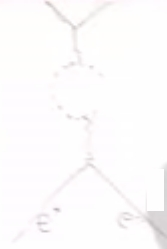
\includegraphics{particles3-2-superpartners}
\end{figure}

Superpartners are expected to be unstable, so we must make them. But one might be stable--dark matter? \glsdesc{gls:LSP}, \gls{gls:LSP}, is likely to be uncharged.

Is the coupling constant stopping us from seeing superpartners?

\begin{figure}[H]
	\caption{Is the coupling constant stopping us from seeing superpartners?}
	\begin{subfigure}[t]{0.45\textwidth}
		\caption{Electron and Superpartner. Will they cancel? Yes.}\label{fig:particles3-2-2loops}
		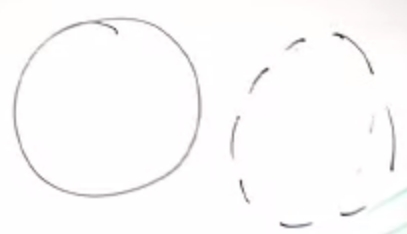
\includegraphics[width=\textwidth]{particles3-2-2loops}
	\end{subfigure}
	\begin{subfigure}[t]{0.45\textwidth}
		\caption{Add photon. Will they cancel? Only if charges of electron and super partner are equal. Otherwise there will be a big discrepency that will lead to a divergent answer.}\label{fig:particles3-2-2loops-photons}
		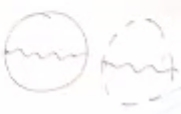
\includegraphics{particles3-2-2loops-photons}
	\end{subfigure}
\end{figure}

It is important that you follow through and ensure that things match at every level.

The super partner of a photon would be have mass. Supersymmetry is not an exact theory.

\begin{itemize}
	\item Superpartner of a Boson is an "-ino": e.g. the superpartner of a photon is a photino, graviton gravitino.
	\item Superpartners of Fermions, have prefix "S-", e.g. Selectron, squark.
\end{itemize}

What would the World be if it were supersymmetric? Would Chemistry \& biology work?

Atoms have electrons. There would be partners to photons and electrons--photinos and selectrons. Now chemistry is what valence electrons do. They are stuck in the outermost shell because of the Pauli Exclusion principle. If we had perfect sypersymmetry, electyron can emit a photino and turn into a selectron. Being a Boson the selectron can then drop to lower energy levels. We'd end up with a Bose-Einsteain condensate of selectrons.


\section{Propagators and renormalization of mass}

We will go back over some of the motivations, and repeat some things about divergences that have to do with the renormalization of particles.

A lot of particle physics is dependent on Feynman diagrams. We use them to calculate scattering probabilities: particles go in and go out. Feynman diagrams do this very efficiently. You have to sum all the Feynman diagrams that go into the calculation. Another thing Feynman diagrams do is to help you calculate the effective Lagrangian, 

\begin{defn}[Effective Lagrangian]
	An approximate Lagrangian that is effective at removing a lot of the complexity that was to complicated to calculate. An effective Lagrangian typically involves a cutoff, a smallest distance or a largest momentum.
\end{defn}

The value of a Propagator is the amplitude of putting in a particle at one place and taking it out at another place. Propagators are functions of relative coordinates, $\Delta^\mu$. The propagator can also be Fourier transformed, and expressed as a function of 4 other variables, the Fourier conjugate coordinates, i.e. momentum. The Feynman rules are usually expressed in terms of momentum, but we're not going to do that. In momentum space Feynman diagrams become integrals over momentum. We can think of the Feynman Diagram of Figure \ref{fig:particles3-3-feynman-loop} in two ways:
\begin{itemize}
	\item a propagator joining a point with itself;
	\item an integral over all the momenta that can flow around in this closed loop.
\end{itemize}

\begin{figure}[H]
	\begin{center}
		\caption{Simplest Feynman Diagram -- a closed loop with nothing going in or out. It can be thought of as a propagator joining a point with itself.}\label{fig:particles3-3-feynman-loop}
		\feynmandiagram{a[particle=\( \boldsymbol{\cdot} \)]
			--[scalar,half left]b
			--[scalar,half left]a
		};
	\end{center}
\end{figure}

Feynman diagrams are always sums over all things that can happen. We can think of the divergences as happening in two ways. Either:
\begin{itemize}
	\item because the two points are too close together, being the same point, or;
	\item there are too many momenta to integrate over.
\end{itemize}

Momentum is associated with inverse wavelength, so large momentum is small wavelength. We can think of diagram being in $\vec{k}$ space or $\vec{x}$ space.

What is the propagator between two points for various kinds of particles?

\begin{figure}[H]
	\caption[Propagators between two points for various kinds of particles.]{Propagators between two points for various kinds of particles. There are two points shown, to emphasize dependence on $x$ and $y$}
	\begin{subfigure}[t]{0.3\textwidth}
		\caption{Spin 0}
		\feynmandiagram{a[particle=\( \boldsymbol{\cdot} \boldsymbol{\cdot} \)]
			--[scalar,half left]b
			--[scalar,half left]a
		};
	\end{subfigure}
	\begin{subfigure}[t]{0.3\textwidth}
		\caption{Spin $\frac{1}{2}$}
		\feynmandiagram{a[particle=\( \boldsymbol{\cdot} \boldsymbol{\cdot} \)]
			--[fermion,half left]b
			--[fermion,half left]a
		};
	\end{subfigure}
	\begin{subfigure}[t]{0.3\textwidth}
		\caption{Spin 1}
		\feynmandiagram{a[particle=\( \boldsymbol{\cdot} \boldsymbol{\cdot} \)]
			--[boson,half left]b
			--[boson,half left]a
		};
	\end{subfigure}
\end{figure}

Propagators look like this:
\begin{align*}
	\braket{0|\Phi(x)\Phi(y)|0}& \text{, spin 0--Higgs}\\
	\braket{0|\Phi^\dagger(x)\Phi(y)|0}& \text{, spin 0 charged}\\
	\braket{0|\Psi^\dagger_i(x)\Psi_j(y)|0}& \text{, spin $\frac{1}{2}$ -- 4 component spinor}\\
\end{align*}

\subsection{Scalar Bosons}

Mass is inverse length. So a length scale is also a mass scale. But when you are talking about massless particles the only scale is length: dimensional analysis is enough to give the form of the (value of the) propagator. Once there is a mass, then the answer is a little more complicated.

For the massless case we want to figure out the dimensions of $\Psi$: the basic rule is the action is always dimensionless (because $\hslash=1$).



\begin{align*}
	[\int d^x \big(\frac{\partial \phi}{\partial x}\big)^2] =&[\mathfrak{l}] \text{, or}\\
	[\mathfrak{l}]^2[\phi]^2=&[\mathfrak{l}]\\
	[\phi]=&[\mathfrak{l}]^{-1} \text{, by dimensional analysis. Now let's check}\\
	[\int d^x \big(\frac{\partial \phi}{\partial x}\big)^2 - \underbrace{\frac{m^2}{2}}_\text{$[m]=[l]^{-1}$} \phi^2]=&[\mathfrak{l}]\\
	[\int d^x \big(\frac{\partial \phi}{\partial x}\big)^2 - \frac{m^2}{2}\phi^2 + \lambda \phi^4] =&[\mathfrak{l}] \text{ requires $\lambda$ dimensionless}
\end{align*}

Propagator can only depend on distance between $x$ and $y$ (homogeneity of space), and it has to be Lorentz invariant, so it can only depend on the proper distance between the points, whence:

\begin{align*}
	[\braket{0|\Phi(x)\Phi(y)|0}]=&\frac{1}{\Delta}^2 \text{, to within a numerical constant, where}\\
	\Delta^2 =& \Delta^\mu\Delta_\mu
\end{align*}

What happens when there is a mass in a problem? Here is the logic. As a general rule, things with very large momentum forget that the particle has mass. For example, the energy of a particle with momentum $p$ is:
\begin{align*}
	E =& \sqrt{p^2 + m^2} \text{. What happens if $p$ gets very large}\\
	E \approxeq& \lvert p \rvert \text{, with exact equality for a massless particle}
\end{align*} 

This is an example of how a formula forgets mass when $p$ is  large. Large momentum means small mass, so propagators become insensitive to mass at short distances. The Fourier transform of a propagator is a function of momentum, and the high momentum part forgets the mass. But high momentum is intimately connected with short distance. At very short distances, $\frac{1}{\Delta^2}$ is the way the propagator behaves. What is there is mass? How is it corrected? It is corrected by things that can be important at large distances. When $\Delta > \frac{1}{m}$, particle has a harder time propagating a large way. This is why forces mediated by massless particles are longer range than forces mediated by massive particles. So the typical thing that happens approximately is propagator behaves like  $\frac{e^{- \Delta m}}{\Delta^2}$ -- Figure \ref{fig:particles3-3-massive-and-massless-propagators}

\begin{figure}[H]
	\caption{Massive and Massless propagators}\label{fig:particles3-3-massive-and-massless-propagators}
	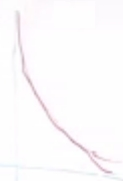
\includegraphics{particles3-3-massive-and-massless-propagators}
\end{figure}

Figure \ref{fig:particles3-3-loops-p} depicts the correction from $\lambda \phi^4$ to the mass term. It gives $\frac{\lambda}{\Delta^2}$, which is infinite for $\Delta=0$. We can't trust our theories for very small distances. We know there is some fuzziness at very small distance, but we know very little about it. 

\begin{figure}[h]
	\begin{center}
		\caption{Correction from $\lambda \phi^4$: 2 particles in and 2 out}\label{fig:particles3-3-loops-p}
		\feynmandiagram[inline=(b.base),vertical=e3 to e1]{
			e1--[scalar]e2--[scalar]e3,
			e2--[scalar,half left]b
			--[scalar,half left]e2
		};$\lambda$
	\end{center}
\end{figure}

If we think of Figure \ref{fig:particles3-3-loops-p} representing an integral over momenta we are getting too much from high momenta. So you could think of a cutoff at small distances or high momenta.

NB $\frac{e^{- \Delta m}}{\Delta^2}$ doesn't help with small $\Delta$.

\subsection{Fermions}

The only difference is the form of the Lagrangian. The action is

\begin{align*}
	\int d^4x \big[\bar{\Psi} \gamma^\mu \partial_\mu \Psi + m \bar{\Psi} \Psi\big]
\end{align*}
which must have dimension 1, giving $[\Psi]=\frac{1}{\mathfrak{l}^\frac{3}{2}}$ (Fermions always have halves!). We find:
\begin{align*}
	[\braket{0|\Psi^\dagger_i(x)\Psi_j(y)|0}]=&\frac{1}{\Delta^3} \text{, or, more exactly,}\\
	=& \big(\frac{\Delta_\mu \gamma^\mu}{\Delta^4}\big)_{ij}
\end{align*}

Recall Figure \ref{fig:particles3-3-loops-p}, and the fact that closed loop diagrams for Bosons are positive, and those for Fermions negative--Theorem \ref{thm:contribution:loops}. Figure \ref{fig:fermion:loop} shows a scalar boson splitting into two Fermions and recombining. The amplitude is:

\begin{align*}
	- g^2 \int d^4 \Delta \frac{1}{\Delta^6}& \text{. introducing the cutoff distance $\delta$}\\
	- g^2 \int_\delta^\infty d^4 \Delta \frac{1}{\Delta^6}&=-\frac{g^2}{\delta^2} \text{, on dimensional grounds.} 
\end{align*}

\begin{figure}[H]
	\begin{center}
		\caption{A scalar boson splitting into two Fermions and recombining, with coupling constants $g$.}\label{fig:fermion:loop}
		\feynmandiagram[vertical=d to a]{
			a--[scalar]b[particle=g]--[fermion,half right,edge label=\(\frac{1}{\Delta^3}\)]c[particle=g]--[scalar]d,
			b--[anti fermion,half left,edge label=\(\frac{1}{\Delta^3}\)]c
		};
	\end{center}
\end{figure}

What are the dimension of $g$? The action is
\begin{align*}
	\int d^4x \big[\bar{\Psi} \gamma^\mu \partial_\mu \Psi + g \phi \bar{\Psi} \Psi\big]
\end{align*}
whence $g$ is dimensionless.

Now we have our amplitude $\frac{\lambda}{\delta^2} - \frac{g^2}{\delta^2}$. You would think it would take a miracle for $g^2=\lambda$, that it would require some magical structure, some special symmetry: that is supersymmetry. This is the sort of thing supersymmetry does: it relates coupling coefficients to make things like this happen. Note that the masses have to match for this to work.


\section{Symmetry and Grassmann numbers}

\subsection{Symmetry}

Symmetries always relate things that are being transformed in some way. Things that are related by symmetries generally have the same mass. Whether supersymmetry is a continuous symmetry or not is a question which has no answer. It doesn't fall into the category of things where the question makes sense.

Symmetries are operations on a system which are described by operators. The system is described by state vectors. Consider a rotation:

\begin{align*}
	U\ket{\psi} \text{, where U is unitary, characterized by axis and angle}
\end{align*}

Any symmetry requires a unitary matrix, $U\dagger U=1$. An infinitesimal unitary transformation has the form:
\begin{align*}
	U =& I + i \epsilon L \text{, where I is Hermitean, e.g. }\\
	=& I + i \underbrace{\epsilon}_\text{angle} \underbrace{L_x}_\text{ab out x axis}
\end{align*}

An important constant is the commutator algebra on the generators, e.g.:
\begin{align*}
	[L_i,L_j] =& i e_{ijk} L_k 
\end{align*}

What is the geometric meaning of the commutator algebra, and the fact that the generators close under commutation? Consider two rotations, $U$ and $V$.
\begin{align*}
	V^\dagger U^\dagger VU \ne& I \text{, except for a few special values of $U$ and $V$, but}\\
	V^\dagger U^\dagger VU =& W \text{, some other rotation.}
\end{align*}

Let's try small rotations:
\begin{align*}
	&(I-\underbrace{i\delta L_y}_\text{a}) (I-\underbrace{i\epsilon L_x}_\text{b}) (I+\underbrace{i\delta L_y}_\text{c}) (I+\underbrace{i\epsilon L_x}_\text{d})\\
	= I +& \delta (\underbrace{-i L_y}_\text{a} + \underbrace{-i L_y}_\text{c}) + \epsilon (\underbrace{-i L_x}_\text{b} + \underbrace{-i L_y}_\text{d}) \\
	+& \delta^2 \underbrace{\cancel{(-i^2)} L_y^2}_\text{ac} + \epsilon^2 \underbrace{\cancel{(-i^2)} L_x^2}_\text{bd}\\
	+& \delta \epsilon ( \underbrace{i^2 L_y L_x}_\text{ab}  - \underbrace{i^2 L_y L_x}_\text{ad} -\underbrace{i^2 L_x L_y}_\text{bc} + \underbrace{i^2 L_y L_x}_\text{cd})\\
	+& \text{ ...}\\
	\approxeq  I +& \delta^2 L_y^2 + \epsilon^2 L_x^2 +[Lx,Ly] \text{, to 2nd order.}
\end{align*}

The commutator is the thing that keeps track of the fact that rotations in different order don't cancel out. Whenever you have a group of transformations to whole structure is there in the commutator algebra. You can build any transformation out of a lot of little ones, so if you know how the little ones behave you can figure out the rest.

Generators of rotations are angular momentum; generators for translations are ordinary momentum ($U=I + i \epsilon P_x$), and $[P_i,P_j]=0$. Rotations and translations don't commute-Figure \ref{fig:particles3-4-rotation-translation-dont-commute} --$[L_i,P_j]=i \epsilon_{ijk} L_k$. The commutation relations isn't particularly important; what is important is the fact that everything is kept track of by the commutation relations.

\begin{figure}[H]
	\begin{center}
		\caption{Rotations and Translations don't commute}\label{fig:particles3-4-rotation-translation-dont-commute}
		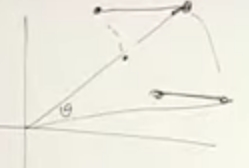
\includegraphics{particles3-4-rotation-translation-dont-commute}
	\end{center}
\end{figure}

If you have a legitimate symmetry group, then the energy should not change when you perform an operation.

\begin{align*}
	H \ket{E} =& E \ket{E}\\
	HU \ket{E} =& E U\ket{E} \text{, if U is a symmetry}\\
	=& U H \ket{E} \text{, whence}\\
	(HU - UH) \ket{E} =& 0 \text{, but the eigenstates are complete, so}\\
	[H,U]=&0 \text{. Now for any generator $L$}\\
	[H,I+i \epsilon L]  =& 0 \text{, or}\\
	[H,L] =& 0 \text{, which implies a conservation law!}
\end{align*}

All the symmetries that we have discussed have one thing in common: they transform Fermions into Fermions, Bosons into Bosons. E.g. a colour symmetry takes a quark to a different coloured quark. They don't affect mass.

Supersymmetry transforms a Boson into a Fermion, and vice versa. It ensures that there is a Fermion for every Boson, and vice versa, and enables us to solve the renormalization issues that we have encountered. The mathematics is very strange.

The generators are called $Q$.

\begin{align*}
	Q \ket{b} =& \ket{f} \numberthis \label{eq:Q:boson}\\
	Q \ket{f} =& \ket{b}
\end{align*}

What kind of operator can do that? We can build one from creation and annihilation operators.

\begin{align*}
	Q =& a^\dagger c + c^\dagger a \\
	(a^\dagger c + c^\dagger a) \ket{b} =& \ket{f}\\
	(a^\dagger c + c^\dagger a) \ket{f} =& \ket{b}\\
	(a^\dagger c + c^\dagger a) \ket{0} = 0 \text{. Doesn't work on vaccum}
\end{align*}

Consider (\ref{eq:Q:boson}) on a scalar Boson: there must be 2 Qs, as Fermion can be up or down, so we need another index, $\frac{\pm 1}{2}$.

\begin{align*}
Q_i \ket{b} =& \ket{f_i} \text{, where $i=\frac{\pm 1}{2}$}\\
Q_i \ket{f_j} =& \ket{b} \text{, if $i=j$}\\
=& 0 \text{ otherwise.}
\end{align*}

The $Q_i$ must have an odd number of Fermion operators; up until now we have worked with things with an even number.

We remind ourselves of some properties of creation and annihilation operators. For Bosons:
\begin{align*}
	[a_i,a_j] =& 0\\
	[a_i^\dagger,a_j^\dagger]=&0\\
	[a,a^\dagger] =& 1\\
	a_i^\dagger a_j^\dagger \ket{0} =& a_j^\dagger a_i^\dagger \ket{0} \text{, symmetry under interchange of Bosons}
\end{align*}

For Fermions:
\begin{align*}
	\{c,c\}=& 0\\
	\{c^\dagger, c^\dagger \}=&0 \text{, Pauli Exclusion pronciple}\\
	\{c, c^\dagger \}=&1\\
	c_i^\dagger c_j^\dagger \ket{0} =& -c_j^\dagger c_i^\dagger \ket{0} 
\end{align*}

The character of Fermions and Bosons is encoded in the commutation and anticommutation relations. The square of a Fermion operator being zero is very different from Bosons. When you build up a large number of Bosons they behave more or less classically. 

There is a generalization of mathematics in which numbers anticommute.



\subsection{Grassmann numbers}

Fermion fields are Grassmann numbers, and so are the generators of Supersymmetry. Grassmann number anticommute.

We start with a collection of ordinary numbers $\{\alpha_i\}$. We know that:
\begin{align*}
	\alpha_j \alpha_j =& \alpha_j \alpha_i
\end{align*}

We invent the Grassmann numbers $\{ \theta_i\}$, with the property:
\begin{align*}
	\{\theta_i,\theta_j\} =& 0 \text{, or}\\
	\theta_i \theta_j =& - \theta_j \theta_i \text{, whence}\\
	\theta_i^2 =& 0
\end{align*}

Imagine that there were only one Grassmann number, $\theta$, say. We suppose that ordinary numbers commute with Grassmann numbers, $[\alpha,\theta]=0$.

They are a bit like odd and even:
\begin{itemize}
	\item the product of two ordinary numbers is ordinary;
	\item the product of two Grassmann numbers is ordinary;
	\item the product or an ordinary number and a Grassmann number is Grassmann.
\end{itemize}

If there is only one Grassmann number\footnote{To within a 1-D vector space}, the function we can build are limited. E.g.
\begin{align*}
	\alpha& + \beta \theta + \underbrace{\gamma \theta^2}_\text{$=0$} 
\end{align*}

Now suppose there are two\footnote{To within a 2-D vector space}
\begin{align*}
	\alpha& + \beta_1 \theta_1 + \beta_2 \theta_2 + \gamma \theta_1 \theta_2 \text{, where}\\
	\theta_1 \theta_2& \ne 0\\
	(\theta_1 \theta_2)^2& = 0
\end{align*}

If there is only one Grassmann number we can construct exponentials.
\begin{align*}
	e^{\alpha \theta} 	e^{\beta \theta} =& (1+\alpha \theta)(1+\beta \theta)\\
	=& [1+(\alpha + \beta) \theta]\\
	=& e^{(\alpha + \beta) \theta} 
\end{align*}

What about two $\theta$s? We can show:
\begin{align*}
	e^{(\theta_1 + \theta_2)} =& e^{\theta_1}  e^{\theta_2} \text{. Actually we saw in Lecture this isn't true!}
\end{align*}

We can integrate and differentiate Grassmann numbers.
\begin{align*}
	\frac{\partial}{\partial \theta_1} \big(\alpha + \beta_1 \theta_1 + \beta_2 \theta_2 + \gamma \theta_1 \theta_2 \big) =& \beta_1 + \gamma \theta_2\\
	\frac{\partial}{\partial \theta_2} \big(\alpha + \beta_1 \theta_1 + \beta_2 \theta_2 + \gamma \theta_1 \theta_2 \big) =& \beta_2 - \gamma \theta_1
\end{align*}

When you pass derivative though Grassmann number, change sign.

\section{A first supersymmetric model}

TBP

\section{Supersymmetry building blocks}

TBP

\section{Lagrangians that preserve supersymmetry}

TBP

\section{Generalizing supersymmetry to 3+1 spacetime, and \gls{gls:QFT}}

TBP

\section{Supersymmetry breaking and an introduction to grand unified theories}

TBP

\section{\gls{gls:GUT}s, the SU(5) representation, proton decay}

TBP

% glossary: may need command makeglossaries particles3
\printglossaries
\bibliographystyle{unsrt}
\addcontentsline{toc}{section}{Bibliography}
\raggedright
\bibliography{tm}

\end{document}
